\clearpage
\section{1 МЕХАНИЗМ РАБОТЫ NANITE}
Общий механизм работы Nanite состоит из двух этапов:
\begin{enumerate}
    \item предподсчёт --- преобразование исходного меша;
    \item отрисовка результата предпосдчёта в игре.
\end{enumerate}

\subsection*{Предподсчёт}
\subsubsection*{Шаг 1}
Исходный меш должен представлять поверхность замкнутого объёма.
Исходный меш разбивается на стыкующиеся между собой маленькие меши, называемые ,,мешлетами,`` от английского термина meshlet.

Для подобного разбиения используется сегментация графа: вершинам графа соответствуют треугольники исходного меша, а рёбрам --- общие рёбра этих треугольников, вес ребра графа пропорционален длине общего ребра треугольников, которому оно соответствует.

Задача сегментации графа состоит в том, чтобы каждой вершине назначить некоторый сегмент так, чтобы сумма весов всех рёбер, смежных с вершинами разных сегментов, была минимальной.

Итоговым сегментам графа соответствуют исходные мешлеты --- в мешлет входят ровно те треугольники, которые соответствуют вершинам, входящим в соответствующий этому мешлету сегмент.

Размер одного мешлета ограничен сверху, но желательно максимально к этому ограничению приблизиться.
Такое требование обусловлено поддержкой видеокарт, которое будет подробнее объяснено в разделе, объясняющем отрисовку.

Для сегментации Nanite использует METIS --- библиотеку с открытым исходным кодом с набором алгоритмов по сегментации графов.
Алгоритмы, предоставляемые METIS, распараллеливаются, но не предоставляют возможности задать жёсткое ограничение на размер одного сегмента, вместо этого задаётся количество сегментов.
Также эти алгоритмы являются вероятностными и только приближают решение задачи, а не решают её точно.
Из-за этого Nanite задаёт такое количество сегментов, чтобы с достаточной вероятностью ни один из получившихся мешлетов не превышал ограничение по размеру.

\subsubsection*{Шаг 2}
После изначального разбиения меша на мешлеты Nanite строит ациклический направленный граф уровней детализации.
Изначально вершинами этого графа назначаются полученные при разбиении исходного меша мешлеты, рёбер нет, для этих мешлетов записывается нулевая оценка искажения.
Далее рёбра в графе мешлетов будут называться стрелками, чтобы отделить их от рёбер треугольников.
Затем повторяется следующий цикл:
\begin{enumerate}
    \item объединить стоки графа (которые являются мешлетами) по четыре в ,,супермешлеты`` --- наборы треугольников, не обязательно попадающие под ограничения для мешлета;
    \item для каждого супермешлета определить те рёбра его треугольников, которые могут также принадлежать треугольникам других супермешлетов.
    Такой набор рёбер называется ,,швом``;
    \item уменьшить детализацию каждого супермешлета так, чтобы его можно было разбить на два мешлета.
    При этом запрещено менять рёбра (и, соответственно, смежные с ними вершины), входящие в швы.
    Уменьшение детализации называется ,,децимацией``, для супермешлета записывается оценка его искажения при децимации;
    \item разбить каждый супермешлет на два мешлета, которые становятся новыми вершинами графа.
    В каждый из этих мешлетов записывается одинаковая оценка искажения, равная оценке искажения супермешлета при децимации;
    \item от тех мешлетов, из которых был составлен супермешлет, провести стрелки к тем мешлетам, на которые этот супермешлет был разбит.
    Также необходимо скорректировать оценку искажения новых мешлетов (ставших новыми стоками) так, чтобы поддержать следующее свойство: независимо от ракурса при отрисовке оценка искажения монотонно неубывает при проходе по любой стрелке.
    До первой итреации цикла свойство выполняется, т.к. в графе нет стрелок.
\end{enumerate}
Цикл повторяется до тех пор, пока не останется не более двух стоков.
Легко показать, что на каждой итерации цикла количество стоков в графе уменьшается, следовательно, цикл конечен.

Если не разделять супермешлет на два мешлета, а децимировать его до одного, получится дерево мешлетов, а не просто ациклический направленный граф.
Но тогда швы между мешлетами на втором от корня уровне будут обязательно включать швы между группами мешлетов-листьев, которые являются потомками этих мешлетов.
Например, на рисунке~\ref{fig:meshlet-tree-example} шов между мешлетами 5 и 6 будет обязательно включать все общие рёбра между мешлетами 1 и 3, 1 и 4, 2 и 3 и 2 и 4.
При значительной высоте дерева такой шов сам по себе может включать сильно больше вершин, чем допустимо включить в один мешлет.
\begin{figure}
    \centering
    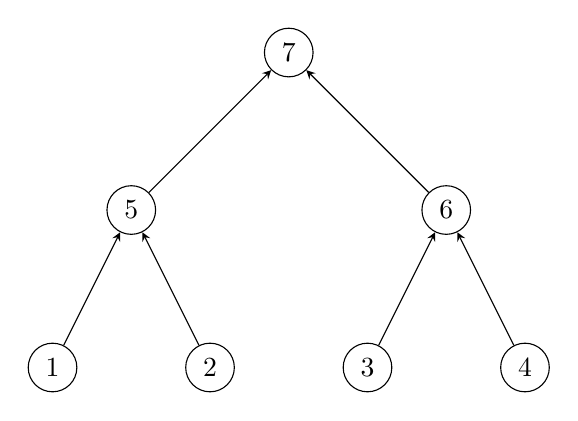
\begin{tikzpicture}
        \node[draw,circle] (m1) at (0,0) {1};
        \node[draw,circle] (m2) at (2,0) {2};
        \node[draw,circle] (m3) at (4,0) {3};
        \node[draw,circle] (m4) at (6,0) {4};
        \node[draw,circle] (m5) at (1,2) {5};
        \node[draw,circle] (m6) at (5,2) {6};
        \node[draw,circle] (m7) at (3,4) {7};
        \draw[->,>=stealth] (m1) -- (m5);
        \draw[->,>=stealth] (m2) -- (m5);
        \draw[->,>=stealth] (m3) -- (m6);
        \draw[->,>=stealth] (m4) -- (m6);
        \draw[->,>=stealth] (m5) -- (m7);
        \draw[->,>=stealth] (m6) -- (m7);
    \end{tikzpicture}
    \caption{Возможное дерева мешлетов}
    \label{fig:meshlet-tree-example}
\end{figure}

Заметим, что мешлеты, полученные при разбиении исходного меша, и только они являются истоками полученного графа.
Далее введём термины для этого ациклического направленного графа, аналогичные терминам на деревьях: если из мешлета $A$ ведёт стрелка в мешлет $B$, то $B$ --- родитель $A$, а $A$ --- ребёнок $B$; если из мешлета $A$ существует путь до мешлета $B$, то мешлет $B$ --- предок мешлета $A$, а $A$ --- потомок $B$.
Тогда свойство графа можно переформулировать так: независимо от ракурса оценка искажения мешлета не превышает оценку искажения его родителя, оценки искажения у родителей одного и того же мешлета равны.

Граф сохраняется вместе с обратными стрелками, т.е. транспонированный граф также доступен.

\subsection*{Отрисовка}
Видеокарты NVidia начиная с серии RTX 2000 и видеокарты AMD начиная с серии RX 6000 поддерживают задание меша для отрисовки не только как массива треугольников, но и как массива мешлетов, при условии ограничения размера мешлетов.
Именно ради этого в предподсчёте появляется требование жёсткого ограничения размера мешлетов.

Благодаря свойству графа, решение о том, рисовать ли конкретный мешлет можно принять независимо для всех мешлетов: мешлет считается подходящим по точности тогда и только тогда, когда его собственная оценка искажения с учётом ракурса ниже определённого порога, а оценка его родителя превышает этот порог.
Если мешлет является стоком, то считается, что оценка его родителя превышает порог.

Такой метод определения гарантирует следующие свойства:
\begin{enumerate}
    \item для каждого мешлета-истока либо он, либо какой-то из его предков будет подходящим по точности;
    \label{nanite-render-trait-1}
    \item для каждого мешлета, подходящего по точности, ни один из его предков или потомков не является подходящим по точности;
    \label{nanite-render-trait-2}
    \item нигде нет щелей между отрисовываемыми треугольниками, через которые можно было бы увидеть внутренний объём меша.
\end{enumerate}

Мешлет, подходящий по точности, всё ещё может не быть отправлен на отрисовку, например, если его описывающий объём не пересекает область видимости.

Свойства \ref{nanite-render-trait-1} и \ref{nanite-render-trait-2} позволяют вместо обхода всех мешлетов использовать обход транспонированного графа от его истоков --- так, если найден мешлет, подходящий по точности, то переходить к его потомкам (в транспонированном графе --- предкам) не имеет смысла.

Алгоритмы растеризации, применяемые в видеокартах, на это не рассчитаны: часто им необходимы производные по экранным координатам от промежуточных результатов вычислений, для вычисления этих производных шейдер --- программа для видеокарты --- запускается минимум на квадрате 2 на 2 пикселя.
Это в 4 раза увеличивает количество вычислений для тех треугольников, которые сами проецируются только на 1 пиксель экрана.

Nanite рассчитан на отрисовку мешлетов столь высокой детализации, что значительная часть треугольников оказывается размером в 1 пиксель.
Чтобы избежать лишних вычислений, Nanite использует вычислительные шейдеры вместо встроенной в видеокарту растеризации.
